\documentclass[]{foi} 
% zakomentirati za pisanje rada na engleskom jeziku
% comment the above line if writing in English

% \documentclass[english]{foi} 
% odkomentirati za pisanje rada na engleskom jeziku
% uncomment the above line if writing in English

\usepackage[utf8]{inputenc}
\usepackage{lipsum}
\usepackage{rotating}
\usepackage{float}

\vrstaRada{\seminar}
% \zavrsni ili \diplomski ili \seminar ili \projekt
% type of the paper:
% \seminar is a seminar/term paper
% \projekt is a project

\title{Rent-a-car}
\predmet{}
% ostaviti prazno ako \vrstaRada nije \projekt ili \seminar
% \predmetBP ili \predmetDP ili \predmetTBP ili \predmetVAS
% leave it empty if \vrstaRada is not a \projekt or \seminar
% \predmetBP - Databases 1
% \predmetVAS - Multiagent Systems

\author{Petar Matišić} 
% ime i prezime studenta/studentice
% name and surname of the author
\spolStudenta{\musko} 
% \zensko ili \musko
% student's gender for grammar purposes: \zensko = F or \musko = M

\mentor{Bogdan Okreša Đurić}
% ime i prezime mentora
% name and surname of the mentor
\spolMentora{\musko} 
% \zensko ili \musko
% mentor's gender: \zensko = F or \musko = M
\titulaProfesora{dr. sc.}
% HR: dr. sc.  / doc. dr. sc. / izv. prof. dr. sc. / prof. dr. sc. 
% mentor's title:
% EN: -prazno- / Asst. Prof.  / Assoc. Prof.       / Full Prof.

\godina{2023}
\mjesec{siječanj}
% mjesec obrane rada ili projekta
% year and month of the presentation of the project or paper

\indeks{0016145882}
% broj indeksa ili JMBAG
% author's ID

\smjer{Informacijsko i programsko inženjerstvo}
% (ili:
%     Informacijski sustavi, 
%     Poslovni sustavi, 
%     Ekonomika poduzetništva, 
%     Primjena informacijske tehnologije u poslovanju, 
%     Informacijsko i programsko inženjerstvo, 
%     Baze podataka i baze znanja, 
%     Organizacija poslovnih sustava, 
%     Informatika u obrazovanju
% )
% study programme; please enter "Erasmus" for incoming exchange students

\sazetak{Aplikacija za \textit{rent-a-car} je softverski alat koji se instalira na računalo i omogućuje vlasnicima \textit{rent-a-car} tvrtki da upravljaju svojim poslovanjem. Takve aplikacije obično uključuju funkcionalnosti poput evidencije najma vozila, računovodstva, vođenja evidencije o klijentima i vozilima, te generiranja izvješća. One također mogu omogućiti automatizirano obavještavanje klijenata o promjenama u dostupnosti vozila, te olakšati rezervacije putem integracije s web stranicom ili drugim kanalima prodaje. \textit{Desktop} aplikacije za \textit{rent-a-car} pomažu tvrtkama da poboljšaju efikasnost i smanje troškove povezane s upravljanjem najmom vozila.}

\kljucneRijeci{najam, vozilo, baza podataka, PostgreSQL, C\#}



\begin{document}

\maketitle

\tableofcontents

\makeatletter \def\@dotsep{4.5} \makeatother
\pagestyle{plain}



\chapter{Uvod}

Ovaj projektni rad bavit će se modeliranjem baze podataka za \textit{rent-a-car}. \textit{Rent-a-car} je općenito iznajmljivanje vozila. U samome procesu iznajmljivanja vozila javljaju se razni entiteti, među kojima postoje neki odnosi, a o kojima će se nešto više reći u ostalim poglavljima.\\

Kroz ovaj projektni rad bit će opisana teorijska podloga korištenih tehnologija, aplikacijska domena, postupak izrade ERA modela (logički i relacijski model baze podataka) te opis alata za izradu. Zatim će se objasniti korišteni okidači i primjeri upita. Nadalje će biti opisana tehnologija za izradu aplikacije, te prikaz same funkcionalnosti razvijene aplikacije.\\

Pomoć pri izradi upita korištena je knjiga \cite{tbp}. Kod kreiranja okidača korištena je knjiga \cite{tbp}.\\

Za izradu baze podataka i razvoj aplikacije korišteni su sljedeći alati: PostgreSQL \cite{postgres}, C\# \cite{microsoft}, Npgsql \cite{npgsql} te DataGrip 2022.2.5 \cite{datagrip} i Visual Studio 2022 \cite{microsoft}. PostgreSQL ima lokalni poslužitelj koji se pokreće preko DataGrip-a. DataGrip je alat koji služi za modeliranje baze podataka, kreiranje tablica, dodavanja veza među tablicama, kreiranja okidača, izvršavanja upita i dr. Visual Studio 2022 je razvojno okruženje u kojemu je napravljena aplikacija u obliku \textit{Windows} formi.

\chapter{Opis aplikacijske domene}

Domena aplikacije je \textit{rent-a-car}, odnosno iznajmljivanje vozila. \textit{Rent-a-car} je danas sve popularniji, gdje agencije iznajmljuju vozila drugim osobama. Središte aplikacijske domene je najam, na kojeg se vežu neki drugi entiteti poput klijenta, vozila, osiguranja, lokacije, računa.

Popis entiteta:
\begin{itemize}
  \item Najam,
  \item Klijent,
  \item Lokacija,
  \item Račun,
  \item Način plaćanja,
  \item Vozilo,
  \item Kategorija,
  \item Model,
  \item Proizvođač,
  \item Osiguranje.
\end{itemize}

Uz navedene entitete, javlja se još jedan entitet koji je po prirodi veze više na više $(M:N)$, a to je entitet Osiguranje najma. Glavni cilj aplikacije je omogućiti izvođenje operacija unosa, čitanja, brisanja i ažuriranja nad bazom podataka, te izvršavanje nekoliko upita. Bitno je napomenuti kako je poslovna logika same aplikacije napravljena na razini baze podataka koristeći aktivne i temporalne vrste baza podataka kroz funkcije i okidače. Sama aplikacija je izrađena u programskom jeziku C\# u razvojnom okruženju Visual Studio 2022 kao \textit{Windows Forms} aplikacija.

Središte aplikacije čini entitet \textbf{najam}, kojeg određuju datum početka i završetka najma, lokacija gdje će klijent preuzeti vozilo te gdje će ga vratiti iznajmljivaču. Osim toga na entitet najam vežemo i podatke o vozilu, klijentu preko vanjskog ključa na te entitete.

\textbf{Klijenta} čini osoba kojoj se iznajmljuje vozilo, a atributi koji ju određuju su njegova šifra, ime, prezime, datum rođenja, mjesto stanovanja, kontakt broj te broj vozačke dozvole. Uz klijenta drugi važan entitet je i \textbf{vozilo}, a atributi koji ga određuju su registracijska oznaka, godina proizvodnje, kilometraža, boja, datum tehničkog pregleda te vanjski ključevi na model, kategoriju te lokaciju. Nakon završetka najma izdaje se \textbf{račun} korisniku, kojeg određuju atributi ID računa, datum izdavanja, iznos, atribut "iskorišteno" koji označava popust na najam auta na neke periode te vanjski ključ na način plaćanja, koji daje sve potrebne podatke klijentu o plaćanju. Uz sve to postoji i entitet osiguranje, kojeg određuju atributi naziv, opis te polica osiguranja.

\chapter{Teorijski uvod}

\section{Relacijske baze podataka}

Relacijske baze podataka (engl. \textit{Relational database management systems, RDBMS}) \cite{tbp} su softverski sustavi koji se koriste za upravljanje relacijskim bazama podataka. Relacijske baze podataka su strukturirane na način da se podaci pohranjuju u tablicama koje su povezane međusobno vezama.

Svaka tablica sadrži niz redaka i stupaca, a svaki redak predstavlja jedan zapis, a svaki stupac jednu određenu vrstu podatka. Na primjer, u tablici "osobe" može se pohraniti ime, prezime i godine svake osobe. Veze između tablica omogućuju povezivanje podataka iz više tablica te se na taj način mogu dobiti kompleksniji podaci. Dakle, relacije između tablica su uspostavljene pomoću ključeva. Postoje dvije vrste ključeva: primarni ključ i vanjski ključ \cite{tbp}. Primarni ključ je jedinstven i ne smije se ponavljati unutar jedne tablice, dok vanjski ključ povezuje red u jednoj tablici s primarnim ključem u drugoj tablici.

Jedna od glavnih prednosti relacijskih baza podataka je njihova strukturiranost i normaliziranost podataka \cite{tbp}. To znači da su podaci pohranjeni na optimalan način te da se u tablicama ne ponavljaju podaci. To omogućuje lakše ažuriranje i održavanje podataka te se sprječava pojava grešaka. Relacijske baze podataka također omogućuju brzo izvršavanje različitih upita i izvještaja. Jedna od još nekoliko prednosti relacijskih baza podataka je njihov integritet podataka \cite{tbp}. Integritet podataka je mjera točnosti i cjelovitosti podataka u bazi podataka. Relacijske baze podataka omogućuju korištenje integritetnih ograničenja kako bi se osiguralo da se podaci unose ispravno i da se ne gube pri ažuriranjima.

Međutim, relacijske baze podataka imaju i neke nedostatke. Jedan od najčešćih je ograničenost u obradi velikih količina podataka, osobito podataka koji se ne lako mogu strukturirati u tablicama \cite{tbp}. Ako se struktura podataka mijenja, to može zahtijevati promjene u cijeloj bazi podataka, što može biti vremenski zahtjevno i skupo. Također, relacijske baze podataka mogu biti skupe u smislu hardverskih i softverskih zahtjeva te zahtijevaju stručno održavanje i administraciju kako bi se osigurala njihova optimalna radna sposobnost i sigurnost \cite{tbp}. Iako se često koriste u velikim korporativnim okruženjima, postoje i drugi tipovi baza podataka koji mogu biti prikladniji za manja poduzeća ili individualne korisnike.
\newpage

\subsection{Aktivne baze podataka}

Aktivne baze podataka (engl. \textit{Active Databases}) \cite{tbp} su specifičan tip baza podataka koje koriste aktivne pravila za upravljanje podacima i njihovim manipulacijama. Ove baze podataka se razlikuju od tradicionalnih relacijskih baza podataka time što imaju integriranu mehanizam za upravljanje pravilima i događajima, što ih čini pogodnim za rješavanje složenih poslovnih zadataka.

Takve vrste baze podataka su programirane da reagiraju na specifične događaje koji se događaju unutar same baze podataka ili u okruženju u kojem se baza nalazi. Ovaj pristup bazama podataka omogućuje im da proaktivno djeluju na temelju događaja i podataka koji su im dostupni, bez potrebe da ih prvo pozove program koji koristi tu bazu podataka \cite{tbp}.

Primjeri događaja koji mogu pokrenuti aktivnost u aktivnoj bazi podataka uključuju promjenu podataka u bazi, dostupnost određenih podataka, vrijeme ili specifičnu akciju korisnika. Na primjer, aktivna baza podataka može imati pravilo da automatski pošalje poruku e-pošte svima koji su zainteresirani za promjenu cijene određenog proizvoda u bazi podataka.

Aktivne baze podataka imaju nekoliko prednosti u odnosu na tradicionalne relacijske baze podataka. Oni omogućuju bolju automatizaciju poslova i smanjuju potrebu za ručnim intervencijama, što može dovesti do ušteda vremena i smanjenja pogrešaka. Također, aktivne baze podataka mogu biti bolje prilagođene specifičnim potrebama korisnika jer mogu reagirati na specifične događaje na način koji je programiran od strane korisnika \cite{tbp}.

Međutim, aktivne baze podataka također imaju neke nedostatke. Jedan od najvećih je složenost njihovog razvoja i održavanja, što može biti skupo i zahtijevati visoko stručne radnike. Također, aktivne baze podataka ne podržavaju sve standarde SQL-a, što može otežati integraciju s drugim sustavima \cite{tbp}. Pored toga, aktivne baze podataka često imaju ograničenja u pogledu veličine i performansi, što ih čini manje pogodnima za velike aplikacije ili one koje zahtijevaju visoku razinu performansi. Iako imaju neke nedostatke, aktivne baze podataka i dalje imaju svoje mjesto u razvoju aplikacija i mogu biti korisne u određenim okolnostima.
\newpage

\subsection{Temporalne baze podataka}

Temporalne baze podataka \cite{tbp} su vrsta relacijskih baza podataka koja ima dodatni kapacitet za spremanje i praćenje vremenskih informacija. Ove baze podataka omogućuju korisnicima da spremaju i prate podatke u sklopu vremenskog konteksta, što je korisno u mnogim aplikacijama gdje je važno pratiti kako se podaci mijenjaju kroz vrijeme. Primjeri takvih aplikacija uključuju financijske sustave, zdravstveni sustavi i sustave za upravljanje projektima.

Jedna od glavnih prednosti temporalnih baza podataka je njihova sposobnost da efikasno prate i spremaju podatke o promjenama u vremenu. Omogućuju korisnicima da lako dohvate podatke u određenom vremenskom rasponu ili da prate promjene u podacima tijekom vremena. Također, temporalne baze podataka često imaju bolje mehanizme za povezivanje podataka u vremenu, što olakšava rad s podacima koji su povezani s vremenom.

Međutim, temporalne baze podataka također imaju neke nedostatke. Jedan od najvećih je složenost njihovog razvoja i održavanja, što može biti skupo i zahtjevno. Osim toga, temporalne baze podataka mogu biti otežane u upravljanju, što može dovesti do poteškoća u pristupu i obradi podataka. Također, korištenje temporalnih baza podataka može dovesti do povećanja veličine baze podataka, što može uzrokovati probleme s performansama \cite{tbp}. Sve u svemu, temporalne baze podataka su korisne u specifičnim situacijama, ali se treba pažljivo razmisliti o njihovoj uporabi u širem kontekstu.
\newpage

\subsection{Opis tehnologija korištenih kod izrade projekta}

\textbf{PostgreSQL} \cite{postgres} je jedna od najpopularnijih i najstarijih otvorenih relacijskih baza podataka. Napravljen je 1990. godine i od tada se stalno razvija. Podržava većinu standarda SQL-a i ima mnoge napredne značajke poput podrške za transakcije, indekse, trigere, procedurne jezike, geospacialne podatke i mnogo toga drugog. PostgreSQL se često koristi u komercijalnim aplikacijama, ali također se može besplatno koristiti u svrhu razvoja i testiranja. Ima veliku zajednicu korisnika i razvojnu ekipu koja se trudi održati visok kvalitet i sigurnost baze podataka. Ovaj softverski alat je moguće preuzeti na poveznici:\\ \texttt{\href{https://www.postgresql.org/download/}{https://www.postgresql.org/download/}}

\textbf{C\#} je programski jezik koji je razvijen od strane Microsofta za upotrebu u razvoju aplikacija za Microsoftove platforme, kao što su Windows i .NET \cite{microsoft}. To je jezik visokog nivoa koji se bazira na C i C++, a nudi mnoge modernije karakteristike kao što su tipiziranje varijabli unaprijed i automatsko upravljanje memorijom. C\# se često koristi u razvoju web aplikacija, igara i mobilnih aplikacija te se smatra jednim od najpopularnijih programskih jezika danas.

Integrirano razvojno okruženje \textbf{Microsoft Visual Studio} \cite{microsoft} je alat za razvoj softvera koji omogućuje programerima da razvijaju aplikacije za različite platforme, uključujući Windows, Mac, Android i iOS. Ono pruža sve potrebne alate za pisanje, testiranje i debuggiranje koda, te integriranu podršku za različite programske jezike, uključujući C\#, C++, Python i mnoge druge. Visual Studio također uključuje integraciju s različitim verzionim kontrolama, što olakšava rad u timu na projektima i omogućava lakše održavanje koda. Ovaj softverski alat je moguće preuzeti na poveznici:\\ \texttt{\href{https://visualstudio.microsoft.com/downloads/}{https://visualstudio.microsoft.com/downloads/}}

\textbf{Npgsql} \cite{npgsql} je ADO.NET \textit{provider} za PostgreSQL baze podataka. Omogućuje .NET aplikacijama da se spajaju na i rade s PostgreSQL bazama podataka. Ovaj softverski alat je moguće preuzeti na poveznici:\\ \texttt{\href{https://www.npgsql.org/doc/installation.html}{https://www.npgsql.org/doc/installation.html}}

\textbf{JetBrains DataGrip} \cite{datagrip} je integrirano razvojno okruženje (IDE) za upravljanje različitim vrstama relacijskih baza podataka. Podržava različite vrste baza podataka, uključujući MySQL, PostgreSQL, Oracle i SQL Server. DataGrip sadrži alate za rad s SQL-om, kao što su uređivač upita, debugger i integracija s repozitorijima kontrola izvornog koda. Također ima mogućnost rada s različitim bazama podataka u isto vrijeme, što ga čini pogodnim za razvoj aplikacija koja se temelji na više baza podataka. DataGrip je dostupan za Windows, MacOS i Linux operativne sustave. Ovaj softverski alat je moguće preuzeti na poveznici:\\ \texttt{\href{https://www.jetbrains.com/datagrip/download/}{https://www.jetbrains.com/datagrip/download/}}

\chapter{Model baze podataka}

\section{Prikaz i opis ERA modela}

Na ERA modelu se prikazuje podatkovna struktura objekata i njihovi odnosi, odnosno kardinalnosti. Kardinalnost se postiže različitim vrstama veza između jedne, dvije ili više tablica. Na ERA modelu za Rent-a-car javljaju se binarne veze jedan naprema više, te jedna veza više naprema više.

Nakon što je izrađen ERA model on se pretvara u relacijski model. On je zasnovan na teoriji skupova \cite{tbp}. Relacijska shema sastoji se od naziva i skupa atributa. Prema tome, relacijski model baze podataka za Rent-a-car je sljedeći:

\begin{itemize}
  \item \textbf{najam} (\underline{IDnajam}, datumpocetkanajma, datumzavrsetkanajma, napomena, \textit{idlokacijapreuzimanja}, \textit{idlokacijaostavljanja}, \textit{idvozilo}, \textit{idklijent}, vrijediod, vrijedido),
  \item \textbf{klijent} (\underline{IDklijent}, ime, prezime, datumrodenja, adresa, grad, postanskibroj, kontaktbroj, brojvozackedozvole),
  \item \textbf{vozilo} (\underline{IDvozilo}, registracijskeoznake, godinaproizvodnje, kilometraza, boja, \textit{idlokacijavozila}, \textit{idkategorija}, \textit{idmodel}, pregled),
  \item \textbf{racun} (\underline{IDracun}, datumizdavanja, iznos, \textit{idnajam}, \textit{idnacinplacanja}, iskoristeno),
  \item \textbf{lokacija} (\underline{IDlokacija}, adresa, grad),
  \item \textbf{model} (\underline{IDmodel}, naziv, \textit{idproizvodac}),
  \item \textbf{proizvodac} (\underline{IDproizvodac}, naziv),
  \item \textbf{kategorija} (\underline{IDkategorija}, naziv),
  \item \textbf{nacinplacanja} (\underline{IDnacinplacanja}, naziv, opis),
  \item \textbf{osiguranje} (\underline{IDosiguranje}, nazivosiguranja, opis, polica),
  \item \textbf{osiguranjenajma} (\underline{Idosiguranje}, \underline{Idnajam}).
\end{itemize}

Primarni ključevi su podcrtani, a vanjski ključevi u kurzivu.

U nastavku na slici \ref{fig:era}. je prikazan ERA model za aplikaciju za Rent-a-car. Model sadrži jedanaest entiteta, koji su međusobno povezani. Veze u modelu su $(1:M)$ te $(N:M)$, ternarnih veza nema.

\begin{sidewaysfigure}[htbp]
    \centering
    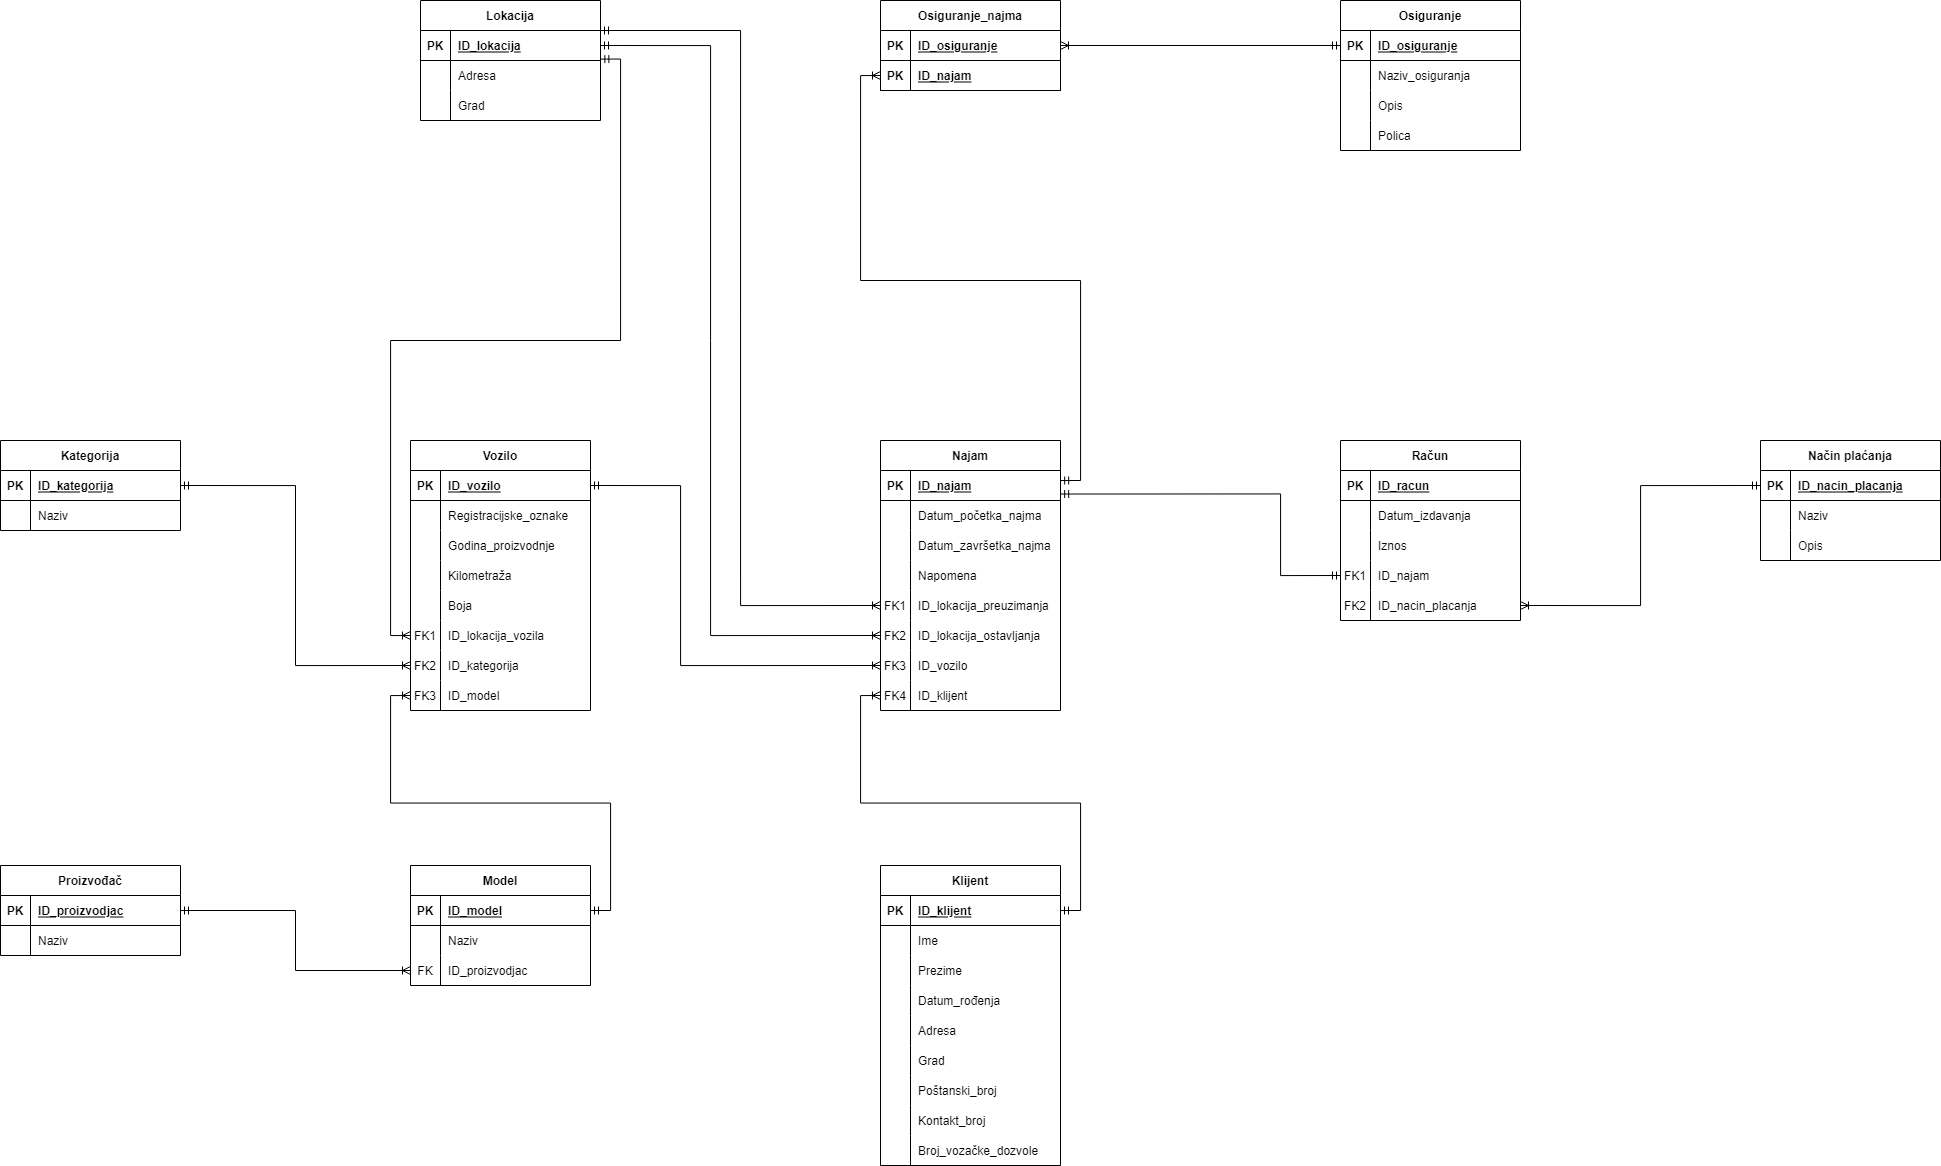
\includegraphics[width=1\textwidth]{slike/era.png}
    \caption{ERA model}
    \label{fig:era}
\end{sidewaysfigure}
\newpage

\subsection{Okidači}

Kod razvoja aplikacije kreirano je osam okidača. Okidači se mogu kreirati u DataGrip-u, a mogu i izravno implementirati u C\# kod. Kod izrade ovoga projekta okidači su kreirani u DataGrip-u na način da se odabere "New Query" te se napiše SQL kod okidača. Nakon što je kreiran, odabere se opcija "Run" te se okidač automatski spremi u mapi "routines" za tablicu za koju je kreiran.\\

\begin{figure}[!ht]
    \centering
    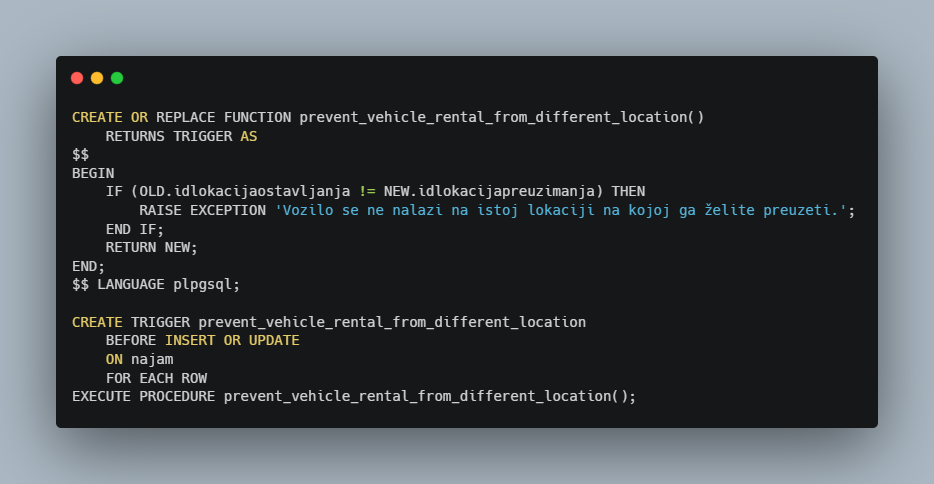
\includegraphics[width=1\textwidth]{slike/1.png}
    \caption{Okidač 1}
    \label{fig:prvi}
\end{figure}

Prvi okidač koji je kreiran sprječava da se unajmi vozilo koje se ne nalazi na istoj lokaciji na kojoj ga klijent želi preuzeti. Ukoliko se lokacija preuzimanja vozila (\texttt{NEW.idlokacijapreuzimanja}) razlikuje od trenutne lokacije vozila  (\texttt{OLD.idlokacijaostavljanja}), okidač će baciti iznimku s porukom \texttt{"Vozilo se ne nalazi na istoj lokaciji na kojoj ga želite preuzeti."}. Inače, okidač vraća nove vrijednosti za "najam". Okidač se izvršava prije \texttt{INSERT} ili \texttt{UPDATE} naredbe na tablici "najam" za svaki redak u tablici.
\newpage

\begin{figure}[!ht]
    \centering
    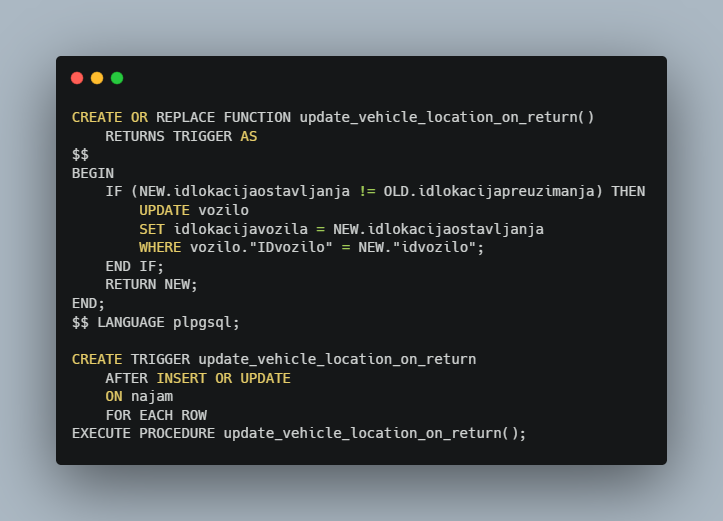
\includegraphics[width=1\textwidth]{slike/2.png}
    \caption{Okidač 2}
    \label{fig:drugi}
\end{figure}

Drugi okidač u PostgreSQL-u koji služi ažuriranju lokacije vozila ukoliko klijent vrati vozilo na neku drugu lokaciju. Ovaj okidač se izvršava nakon unosa ili ažuriranja podataka u tablicu "najam". Ukoliko se lokacija povrata vozila razlikuje od lokacije preuzimanja vozila u tablici, okidač će ažurirati trenutnu lokaciju vozila u tablici "vozilo" tako da se postavi na lokaciju na kojoj je vozilo vraćeno. Okidač vraća nove podatke u tablici "najam".
\newpage

\begin{figure}[!ht]
    \centering
    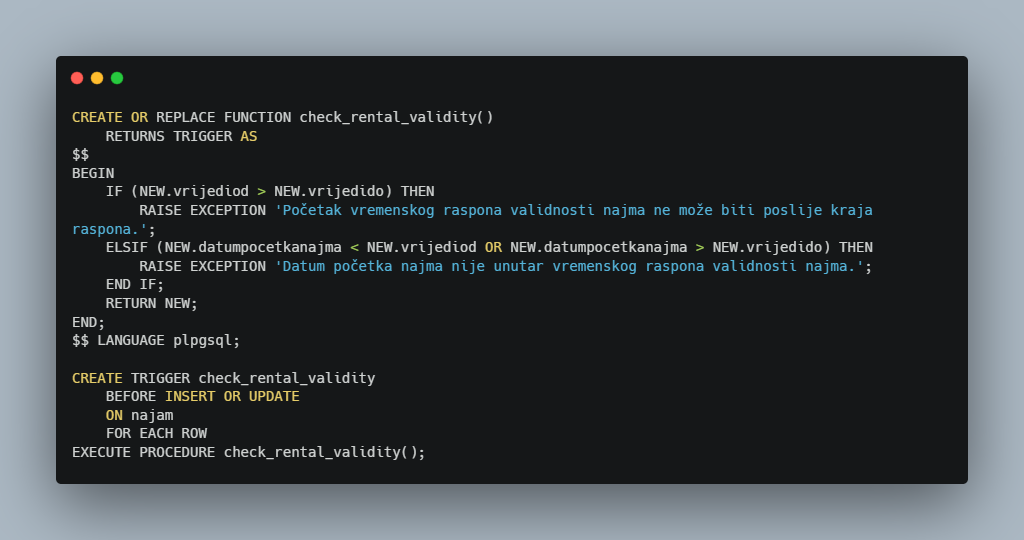
\includegraphics[width=1\textwidth]{slike/3.png}
    \caption{Okidač 3}
    \label{fig:treci}
\end{figure}

Treći okidač \texttt{check\_rental\_validity} provjerava je li vrijeme početka najma unutar vremenskog raspona trajanja najma koji je naveden u tablici "najam". Ako nije, baca iznimku. Ako je početak vremenskog raspona validnosti najma poslije kraja raspona, također baca iznimku. Okidač se izvršava prije svakog INSERT-a ili UPDATE-a u tablici "najam".
\newpage

\begin{figure}[!ht]
    \centering
    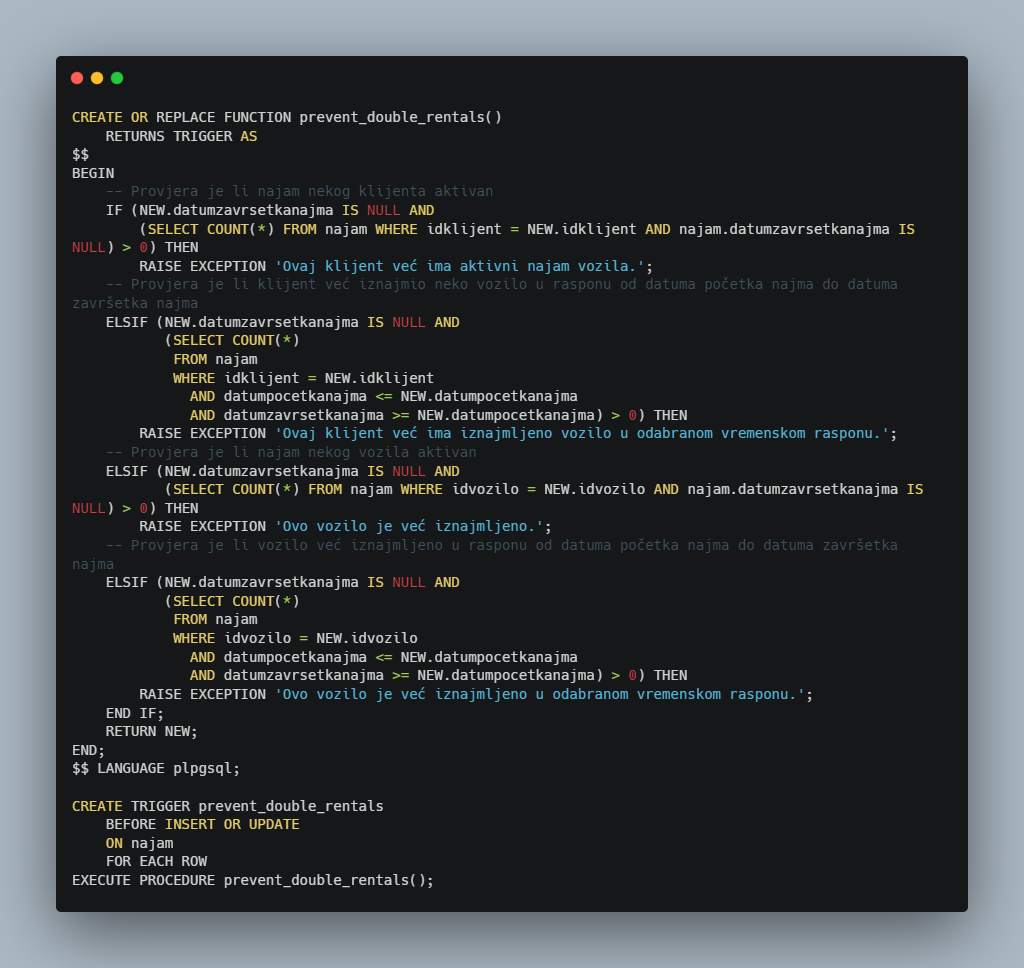
\includegraphics[width=1\textwidth]{slike/4.png}
    \caption{Okidač 4}
    \label{fig:cetvrti}
\end{figure}

Četvrti okidač je namijenjen za provjeru je li se neko vozilo ili neki klijent već nalazi u nekom aktivnom najmu ili da li je vozilo ili klijent već iznajmio neko vozilo, odnosno da se vozilo koristi u nekom zadanom vremenskom rasponu. Ako se bilo koja od tih situacija dogodila, okidač će baciti iznimku s odgovarajućom porukom o grešci. Okidač se izvršava prije unosa ili ažuriranja podatka u tablicu "najam".
\newpage

\begin{figure}[!ht]
    \centering
    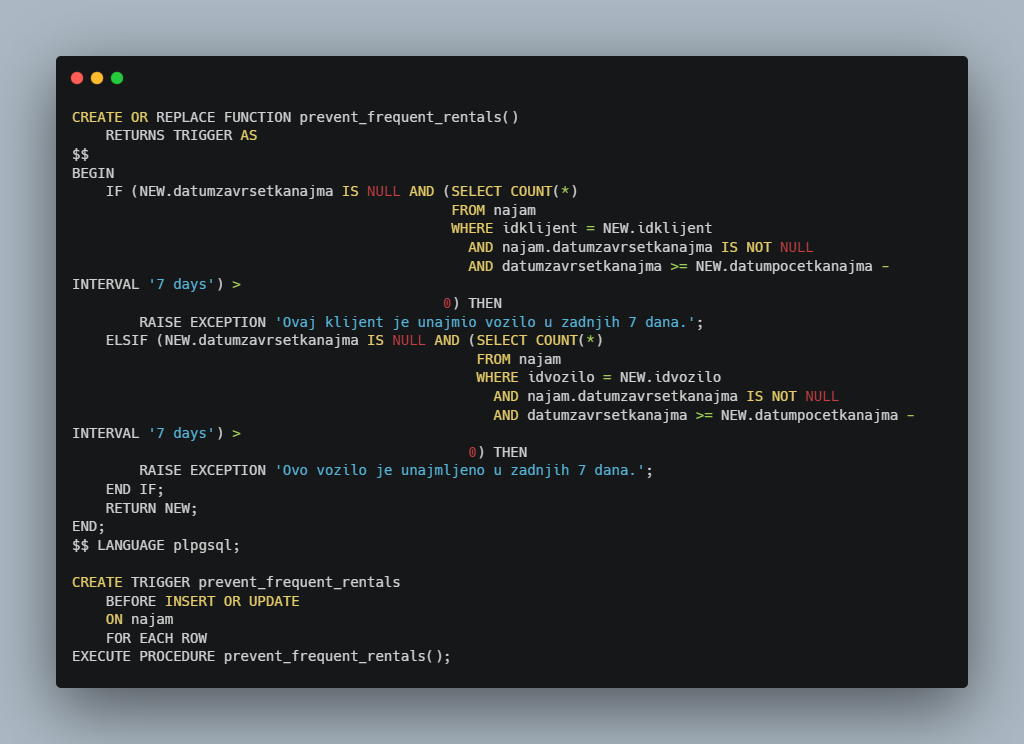
\includegraphics[width=1\textwidth]{slike/5.png}
    \caption{Okidač 5}
    \label{fig:peti}
\end{figure}

Peti okidač se koristi za sprječavanje najma vozila od strane klijenta koji je unajmio vozilo u zadnjih 7 dana ili za sprječavanje najma vozila koje je unajmljeno u posljednjih 7 dana. Okidač se pokreće prije \texttt{INSERT} ili \texttt{UPDATE} naredbe na tabeli "najam" i provjerava je li datum završetka najma prazan. Ako je prazan, okidač provjerava je li postoji zapis u tabeli "najam" s istim ID-om klijenta ili vozila čiji je datum završetka najma nedavno. Ako postoji takav zapis, okidač izbacuje iznimku. Inače, okidač vraća novi zapis.
\newpage

\begin{figure}[!ht]
    \centering
    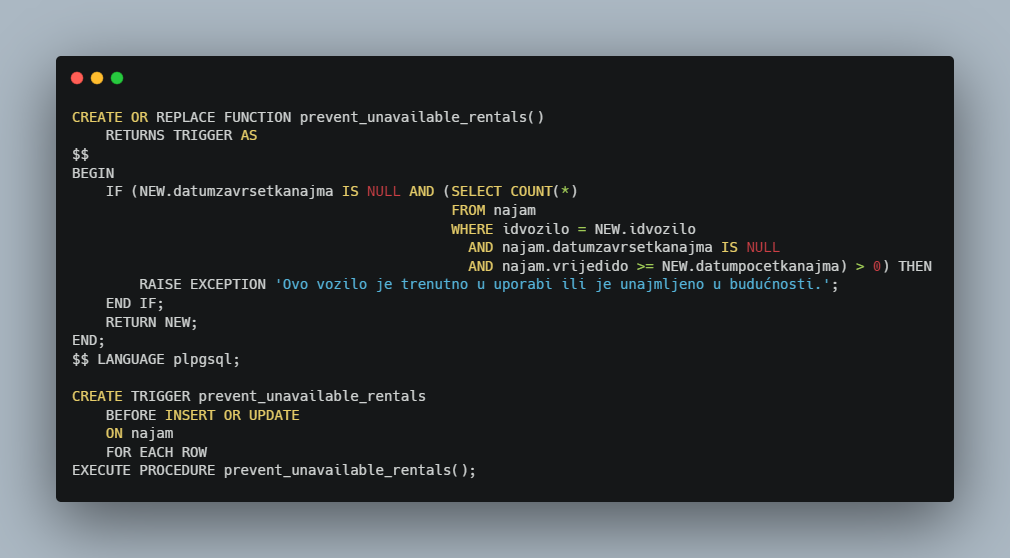
\includegraphics[width=1\textwidth]{slike/6.png}
    \caption{Okidač 6}
    \label{fig:sesti}
\end{figure}

Šesti okidač se poziva prije \texttt{INSERT} ili \texttt{UPDATE} naredbi na tablici "najam" i primjenjuje se na svaki red u tablici. Funkcija \texttt{prevent\_unavailable\_rentals()} provjerava je li vozilo trenutno u uporabi ili je unajmljeno u budućnosti. Ako je vozilo u uporabi ili je unajmljeno u budućnosti, funkcija baca iznimku \texttt{"Ovo vozilo je trenutno u uporabi ili je unajmljeno u budućnosti."}. Inače, vraća novi red u tablici "najam".
\newpage

\begin{figure}[!ht]
    \centering
    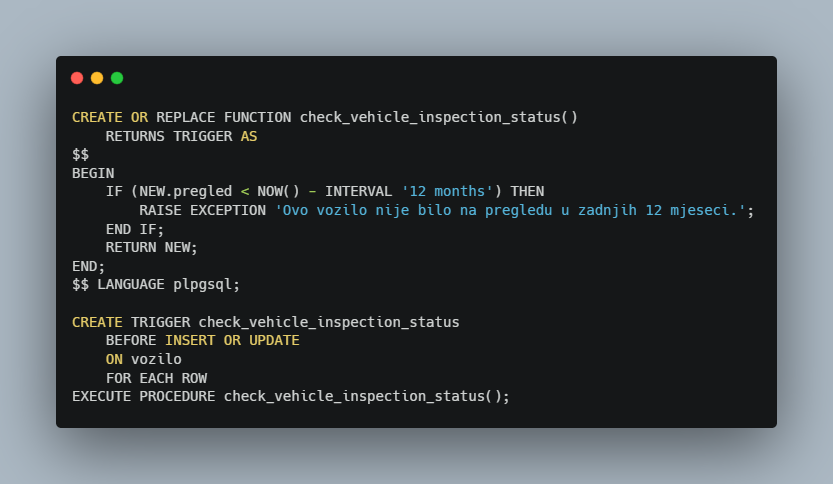
\includegraphics[width=1\textwidth]{slike/7.png}
    \caption{Okidač 7}
    \label{fig:sedmi}
\end{figure}

Sedmi okidač provjerava je li se datum zadnjeg tehničkog pregleda vozila nalazi u posljednjih 12 mjeseci odnosno godini dana. Ako nije, izvršava se naredba \texttt{RAISE EXCEPTION} koja će ispisati poruku o grešci i prekinuti izvršavanje okidača. Inače, okidač vraća nove podatke u tablicu. Okidač se izvršava prije svakog INSERT-a ili UPDATE-a u tablici "vozilo" i to za svaki red u tablici pojedinačno.
\newpage

\begin{figure}[!ht]
    \centering
    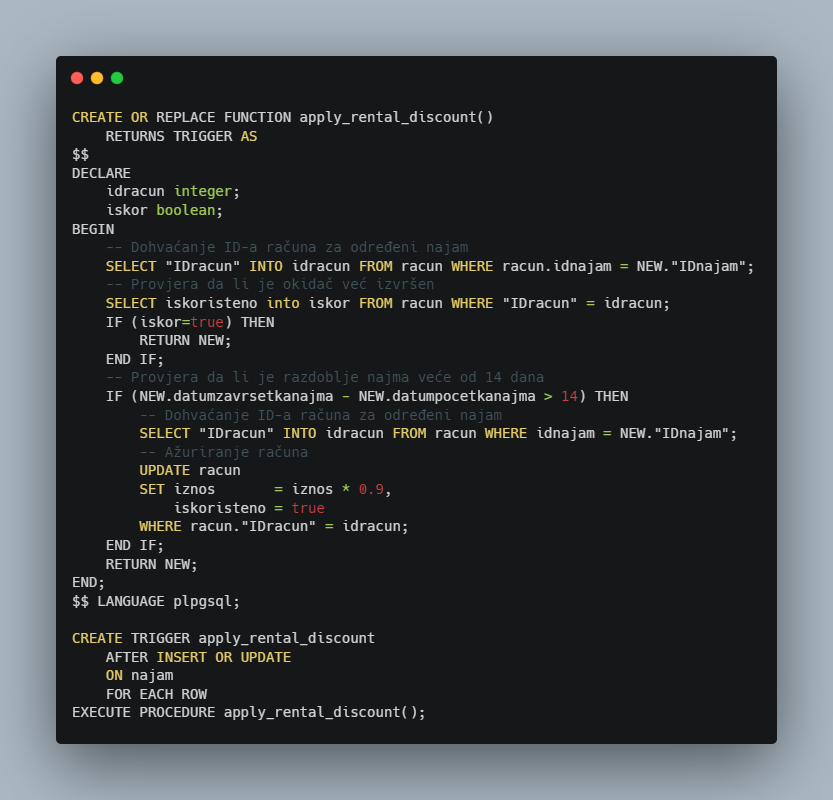
\includegraphics[width=1\textwidth]{slike/8.png}
    \caption{Okidač 8}
    \label{fig:osmi}
\end{figure}

Osmi i zadnji okidač se koristi za primjenu popusta na račun za najam vozila ukoliko je razdoblje najma duže od 14 dana. Okidač prvo dohvaća ID računa za najam koji se promijenio/unio u tablicu "najam" i provjerava je li već primjenjen popust na taj račun. Ako nije, provjerava se da li je razdoblje najma veće od 14 dana. Ako jest, iznos na računu se množi s 0.9 (što predstavlja popust od 10\%) i označava se da je popust primijenjen. Okidač nakon toga vraća nove vrijednosti u tablicu "najam".
\newpage

\subsection{Upiti}

Kod izrade ovoga projekta kreirani su sljedeći upiti:

\begin{itemize}
  \item Upit koji prikazuje datume početka i završetka najma za određeni model vozila,
  \item upit koji prikazuje sva unajmljena vozila, te datume početka i završetka najma za određenog klijenta,
  \item upit koji prikazuje sva vozila koja se trenutno koriste,
  \item upit koji prikazuje sva vozila koja se ne koriste ali za određenu lokaciju.
\end{itemize}

\vspace{20mm}

\begin{figure}[!ht]
    \centering
    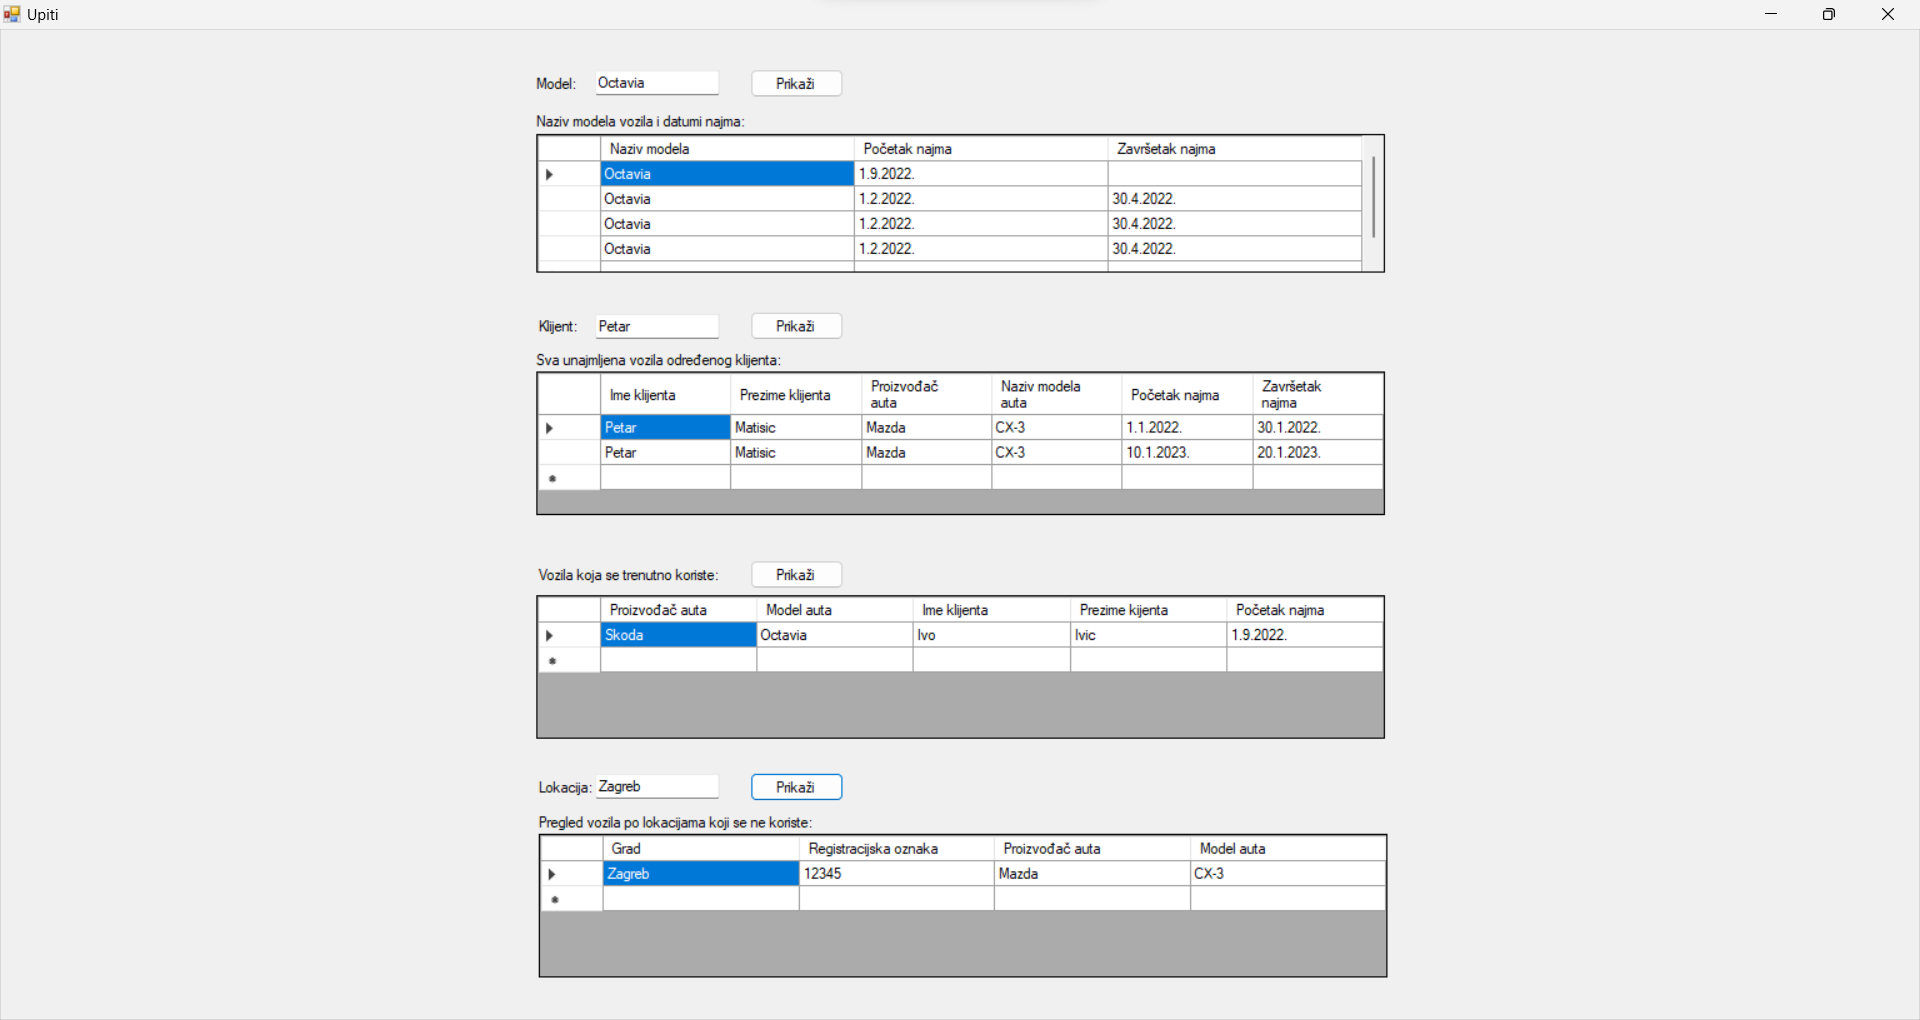
\includegraphics[width=1\textwidth]{slike/upit.png}
    \caption{Windows forma upita}
    \label{fig:upit}
\end{figure}
\newpage

\begin{figure}[!ht]
    \centering
    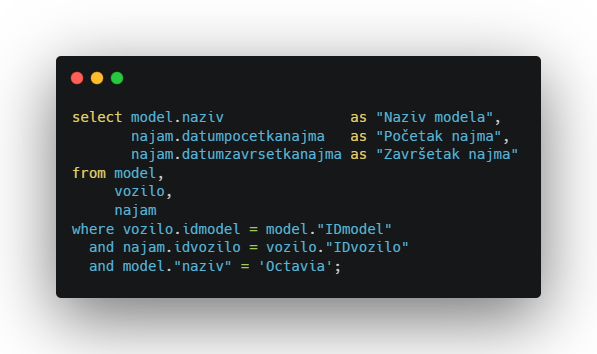
\includegraphics[width=1\textwidth]{slike/u1.png}
    \caption{Upit 1}
    \label{fig:upit1}
\end{figure}

Kod prvog upita u zaglavlju rezultata prikazuje se naziv modela vozila te datum početka i završetka najma. Potrebno je spojiti tablice model, vozilo i najam, izjednačiti vanjske i primarne ključeve, te na kraju primarni ključ tablice model mora biti jednak vrijednosti koju korisnik unese u \textit{textbox} u aplikaciji.

\begin{figure}[!ht]
    \centering
    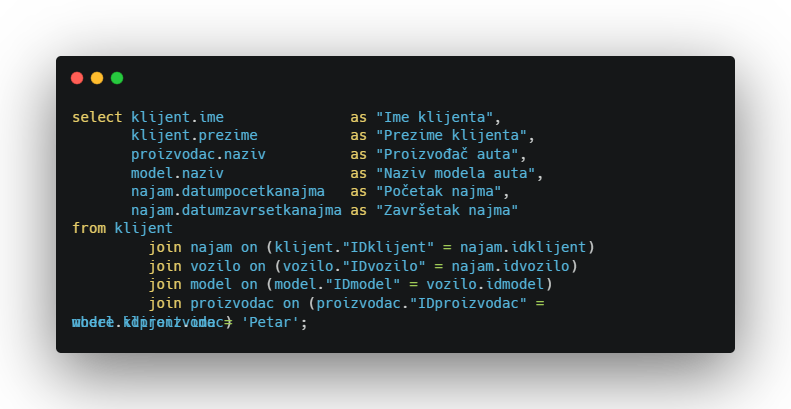
\includegraphics[width=1\textwidth]{slike/u2.png}
    \caption{Upit 2}
    \label{fig:upit2}
\end{figure}

Drugi upit prikazuje sva vozila koje je određeni klijent unajmio. U zaglavlju rezultata upita prikazuju se naziv proizvođača i modela, te datum početka i završetka najma. Spaja se ukupno 5 tablica: klijent, najam, vozilo, model, proizvođač. Izjednačavaju se primarni i vanjski ključevi navedenih tablica te na kraju primarni ključ tablice klijent mora biti jednak vrijednosti upisanoj od strane korisnika u \textit{textbox} u aplikaciji.\\

\begin{figure}[!ht]
    \centering
    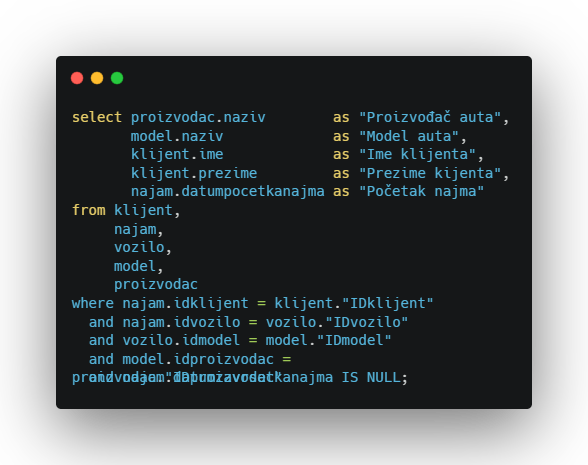
\includegraphics[width=1\textwidth]{slike/u3.png}
    \caption{Upit 3}
    \label{fig:upit3}
\end{figure}

Treći upit koji je kreiran prikazuje nazive modela i proizvođača onih vozila koji se trenutno koriste. U zaglavlju rezultata upita se nalaze nazivi proizvođača i modela, te datum početka najma. Spaja se pet tablica, izjednačavaju se vanjski i primarni ključevi, te na kraju identifikator koristi li se neko vozilo ili ne je datum završetka najma. Ako je polje prazno to znači da se vozilo trenutno koristi.
\newpage

\begin{figure}[!ht]
    \centering
    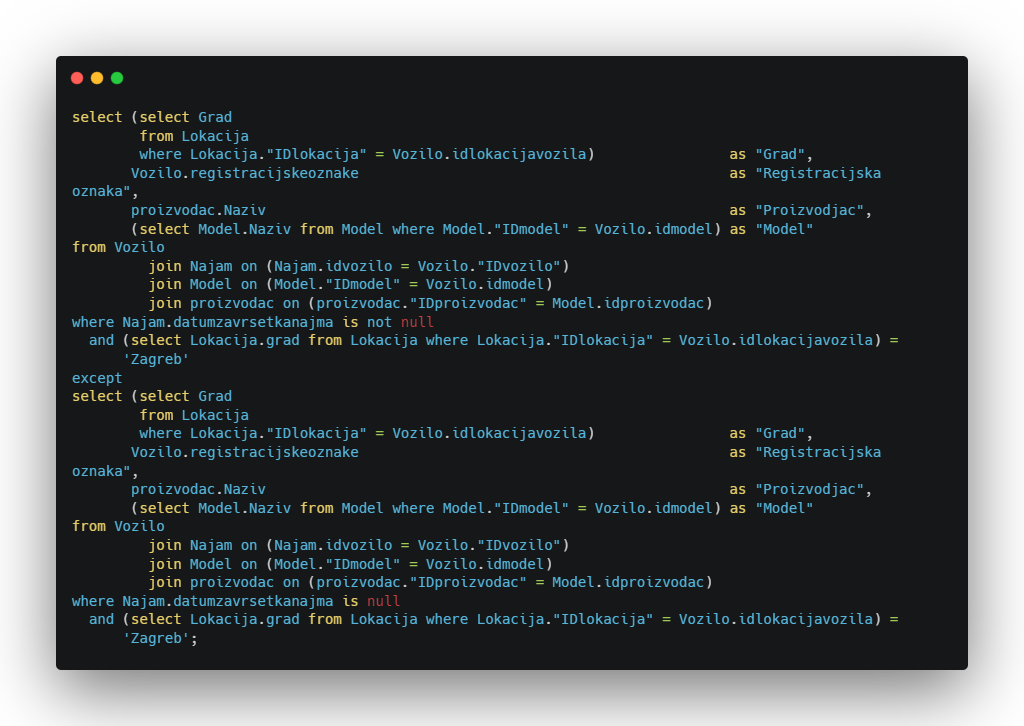
\includegraphics[width=1\textwidth]{slike/u4.png}
    \caption{Upit 4}
    \label{fig:upit4}
\end{figure}

Četvrti kreirani upit vraća sva vozila koja se trenutno ne koriste za određenu lokaciju. U zaglavlju rezultata upita se nalaze naziv grada, registracijska oznaka vozila, kao i naziv proizvođača i modela vozila. Upit sadrži nekoliko podupita: dohvaćanje naziva grada iz tablice Lokacija, dohvaćanje naziva modela iz tablice Model. S obzirom da se iz tablice najam određuje koristi li se neko vozilo ili ne, potrebno je napraviti razliku s obzirom na atribut datum završetka najma.

\chapter{Implementacija i primjeri korištenja}

U ovom su poglavlju prikazane korištene forme za izradu aplikacije. Nadalje, prikazana je jedna implementacija kompletne forme (u ovom slučaju za formu "Najam" jer je ona najkompleksnija), a ostale forme su izrađene na sličan način kao forma "Najam" pa stoga nije potrebno sve ostale opisivati. Forma "Najam" sadrži gumbiće (Kreiraj, Obriši, Ažuriraj, Prikaži) zatim \texttt{textbox}-ove za upis podataka te \texttt{DataGridView} za prikaz podataka. U nastavku je prikazana klasa \texttt{Najam.cs}:
\vspace{5mm}

Prije svega, u linijama 1-7, učitavaju se potrebne biblioteke za rad sa PostgreSQL bazom podataka i grafičkim korisničkim sučeljem.

Nakon toga, u funkciji \texttt{frmNajam\_Load} se otvara konekcija sa bazom podataka i izvršava se SQL naredba za dohvaćanje svih podataka iz tabele "najam". Rezultati se prikazuju u \textit{DataGridView} kontroli \texttt{dgvNajmovi}.

U \textit{event handler}-u \texttt{btnKreiraj\_Click} se otvara konekcija sa bazom podataka i izvršava se SQL naredba za unošenje novog reda u tabelu "najam". Vrijednosti za svako polje se preuzimaju iz odgovarajućih tekstualnih polja. Ako naredba uspije, zatvara se konekcija i poziva se funkcija za prikaz podataka iz tabele najam u \textit{DataGridView} kontroli. U slučaju bilo kakve greške, ista se prikazuje u \textit{MessageBox}-u. Ako se konekcija uspješno otvori, obavezno se zatvara na kraju programskog bloka, a ako je došlo do ikakvih grešaka, tada u \texttt{finally} bloku.

U \textit{event handler}-u \texttt{btnObrisi\_Click} se otvara konekcija sa bazom podataka i izvršava se SQL naredba za brisanje reda iz tabele "najam". Vrijednost za primarni ključ se preuzima iz tekstualnog polja \texttt{tbIDnajma}. Ako naredba uspije, zatvara se konekcija i poziva se funkcija za prikaz podataka iz tabele "najam" u \textit{DataGridView} kontroli. U slučaju bilo kakve greške, ista se prikazuje u \textit{MessageBox}-u. Ako se konekcija uspješno otvori, obavezno se zatvara na kraju programskog bloka, a ako je došlo do ikakvih grešaka, tada u \texttt{finally} bloku.

U \textit{event handler}-u \texttt{btnAzuriraj\_Click} se otvara konekcija sa bazom podataka i izvršava se SQL naredba za ažuriranje postojećeg reda u tabeli najam. Vrijednosti za svako polje se preuzimaju iz odgovarajućih tekstualnih polja. Ako naredba uspije, zatvara se konekcija i poziva se funkcija za prikaz podataka.

Funkcijom \texttt{prikazi\_podatke} dohvaćaju se podatci iz baze \texttt{SELECT} upitom te ih se prikaziva u \textit{DataGridView}-u. Ovu funkciju se poziva u \textit{event handler}-ima \texttt{frmNajam\_Load} i \texttt{btnPrikazi\_Click}.

Forma "Najam" i njeni elementi se mogu pogledati u \hyperref[sec:najam]{sekciji 5.0.6.}
\newpage

\begin{figure}[!ht]
    \centering
    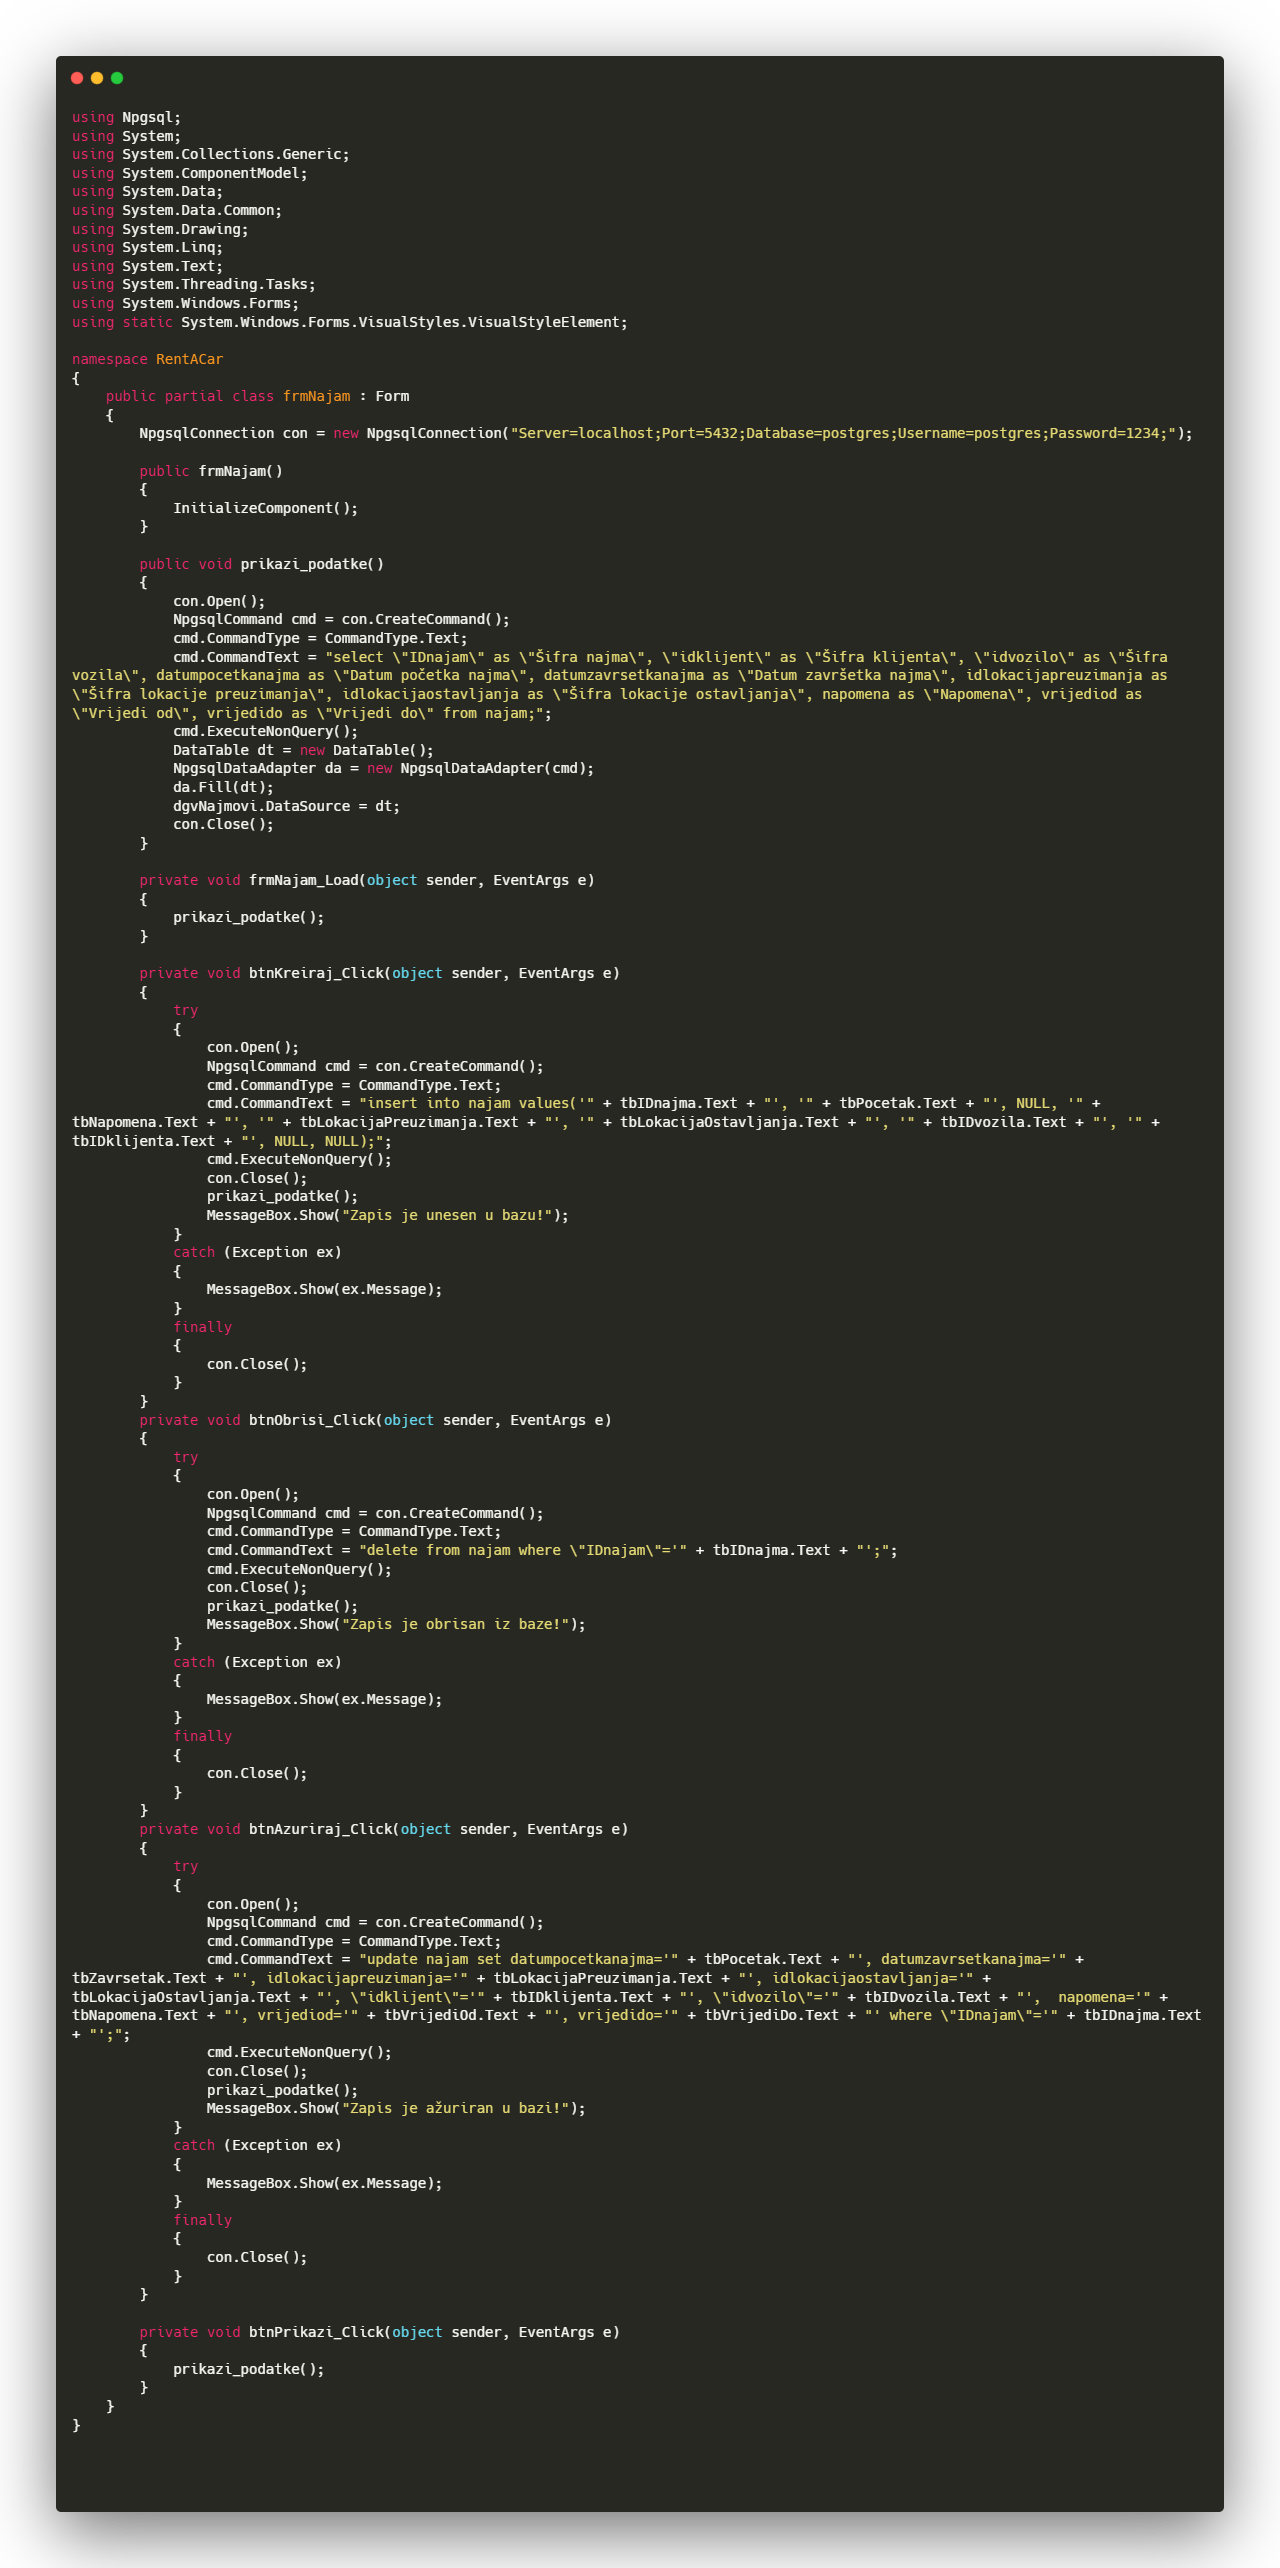
\includegraphics[width=0.73\textwidth]{slike/klasa.png}
    \caption{Klasa Najam.cs forme Najam}
    \label{fig:klasa}
\end{figure}
\newpage

\subsection{Kategorija}

\begin{figure}[!ht]
    \centering
    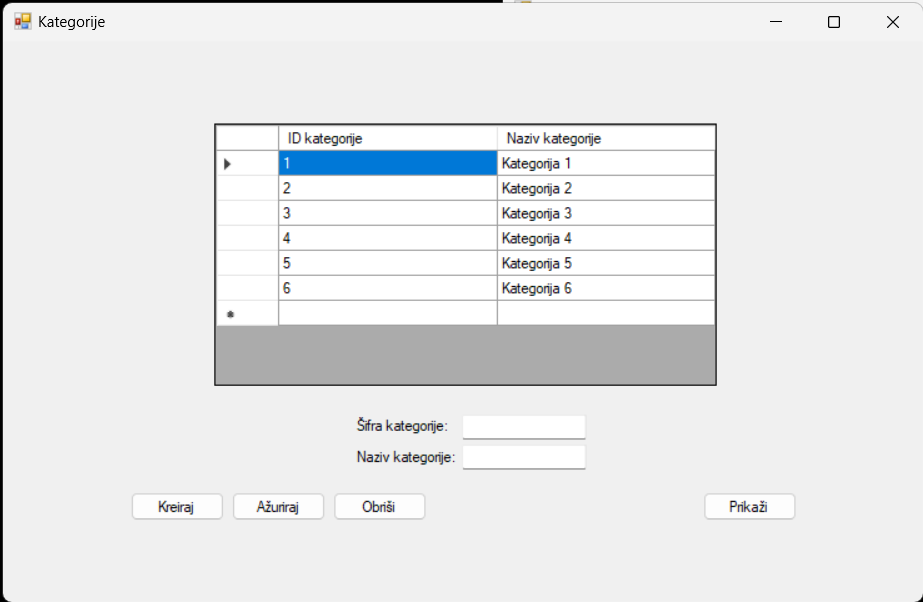
\includegraphics[width=0.9\textwidth]{slike/kategorija.png}
    \caption{Forma Kategorija}
    \label{fig:kategorija}
\end{figure}

\subsection{Klijent}

\begin{figure}[!ht]
    \centering
    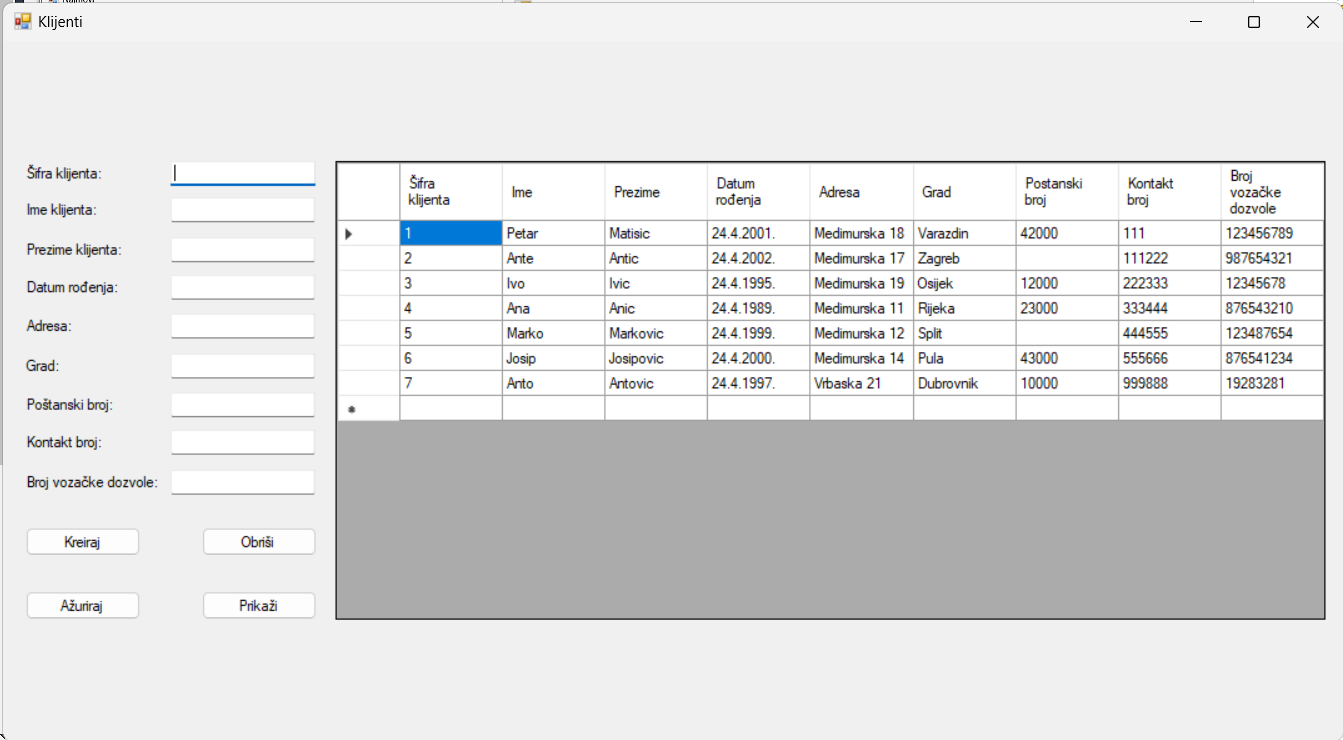
\includegraphics[width=0.9\textwidth]{slike/klijent.png}
    \caption{Forma Klijent}
    \label{fig:klijent}
\end{figure}
\newpage

\subsection{Lokacija}

\begin{figure}[!ht]
    \centering
    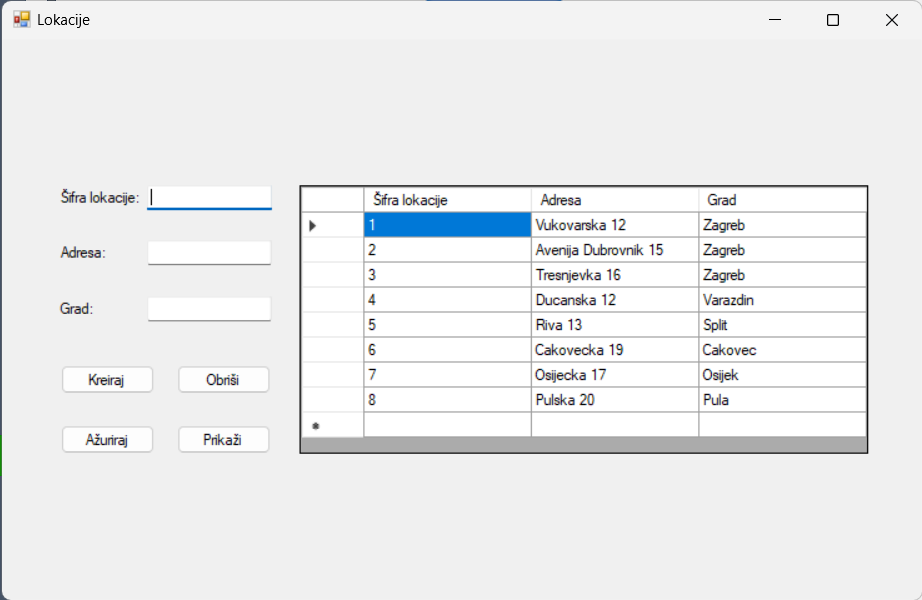
\includegraphics[width=0.9\textwidth]{slike/lokacija.png}
    \caption{Forma Lokacija}
    \label{fig:lokacija}
\end{figure}

\subsection{Model}

\begin{figure}[!ht]
    \centering
    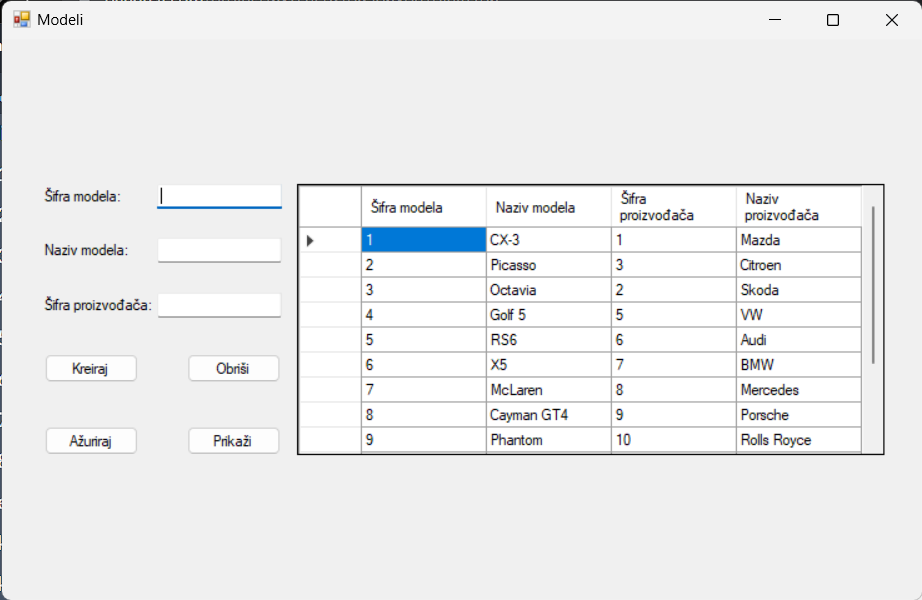
\includegraphics[width=0.9\textwidth]{slike/model.png}
    \caption{Forma Model}
    \label{fig:model}
\end{figure}
\newpage

\subsection{Način plaćanja}

\begin{figure}[!ht]
    \centering
    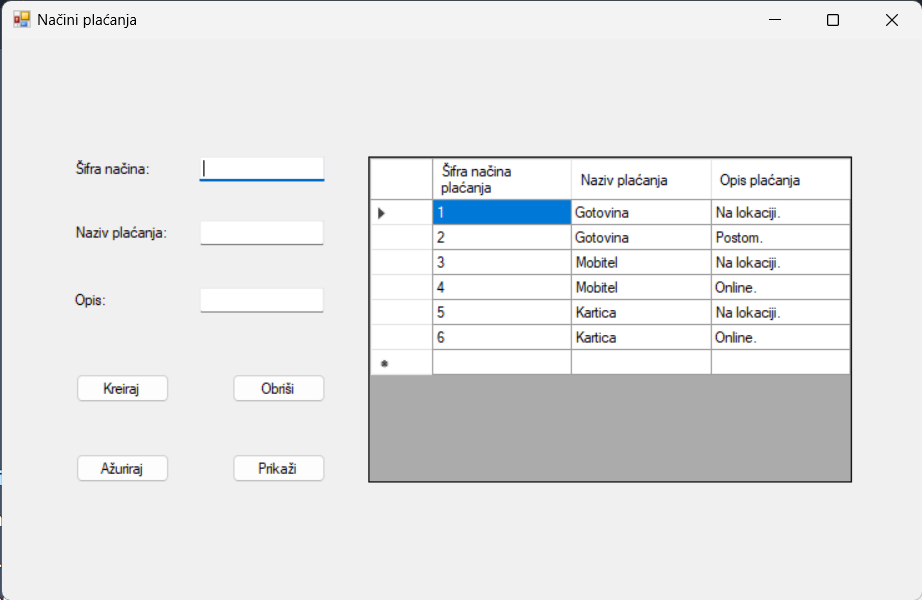
\includegraphics[width=0.9\textwidth]{slike/nacin.png}
    \caption{Forma Način plaćanja}
    \label{fig:nacin}
\end{figure}

\subsection{Najam}
\label{sec:najam}

\begin{figure}[!ht]
    \centering
    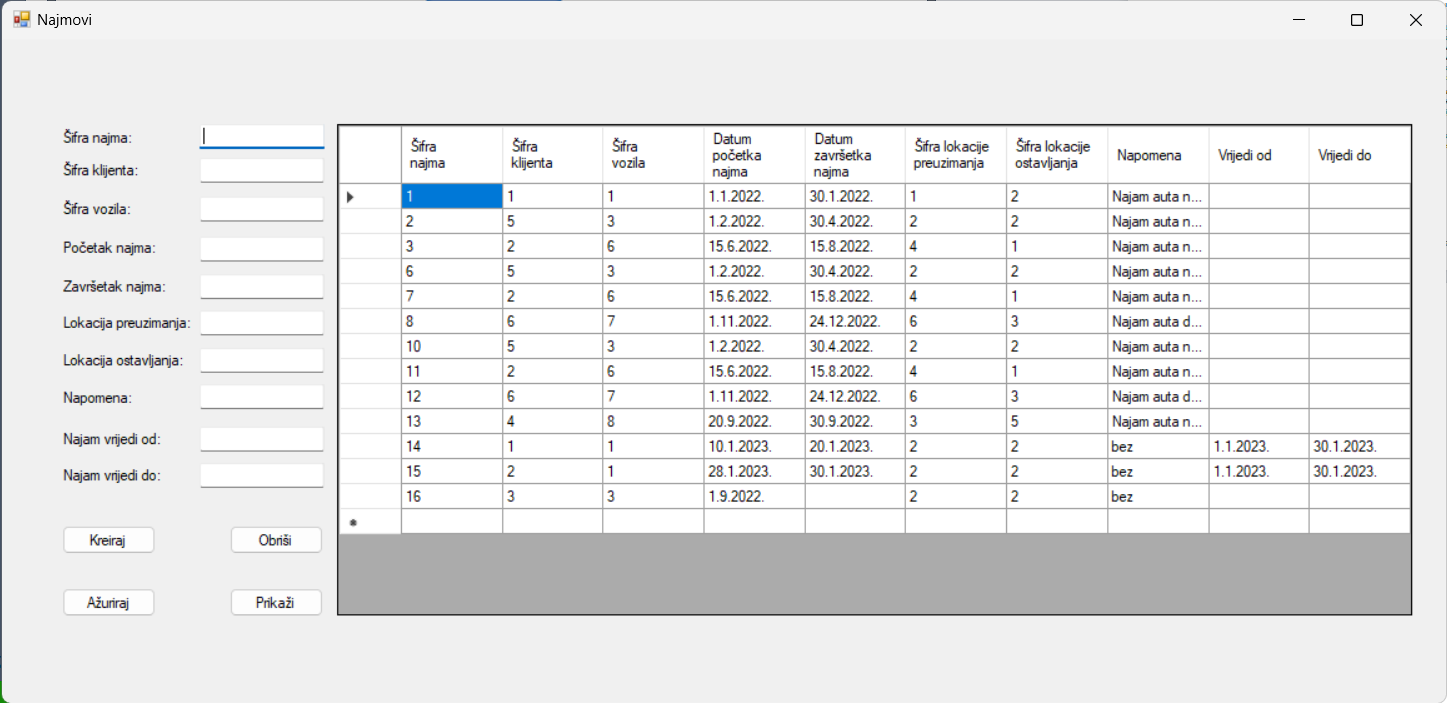
\includegraphics[width=0.9\textwidth]{slike/najam.png}
    \caption{Forma Najam}
    \label{fig:najam}
\end{figure}
\newpage

\subsection{Osiguranje}

\begin{figure}[!ht]
    \centering
    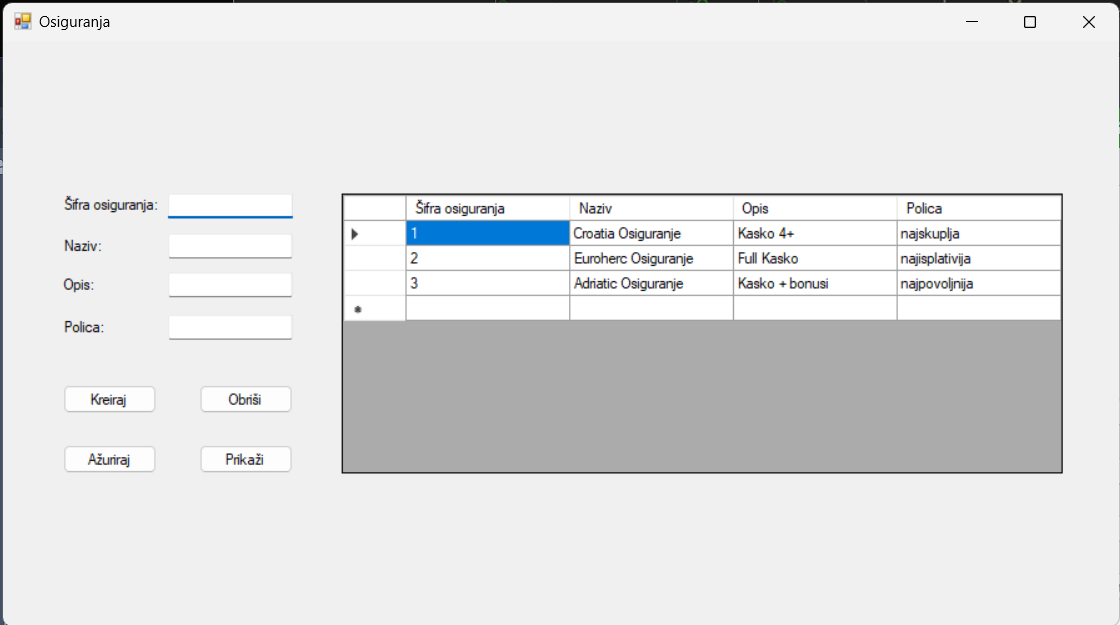
\includegraphics[width=0.9\textwidth]{slike/osiguranje.png}
    \caption{Forma Osiguranje}
    \label{fig:osiguranje}
\end{figure}

\subsection{Osiguranje najma}

\begin{figure}[!ht]
    \centering
    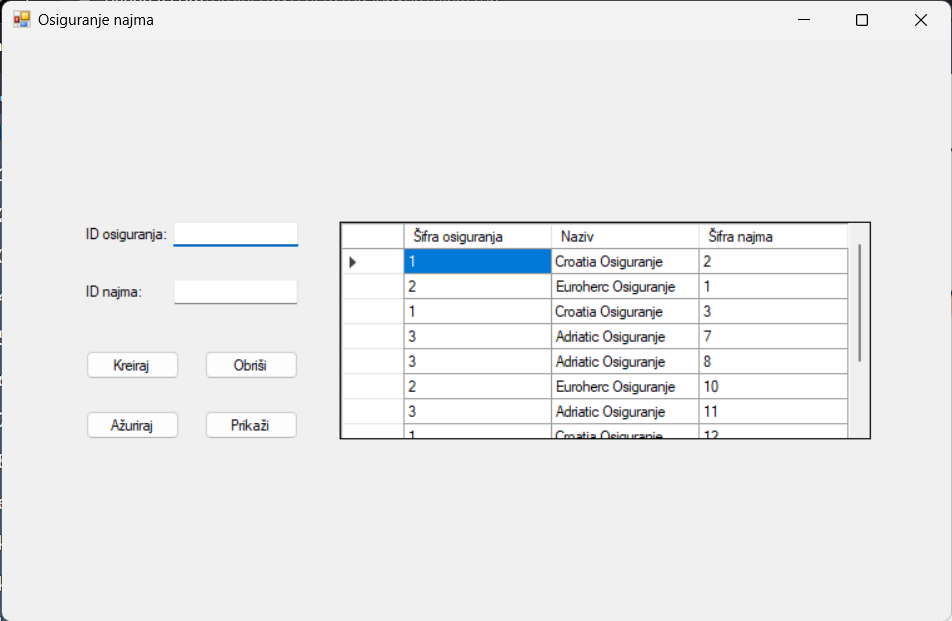
\includegraphics[width=0.9\textwidth]{slike/osiguranjenajma.png}
    \caption{Forma Osiguranje najma}
    \label{fig:osiguranjenajma}
\end{figure}
\newpage

\subsection{Početna stranica}

\begin{figure}[!ht]
    \centering
    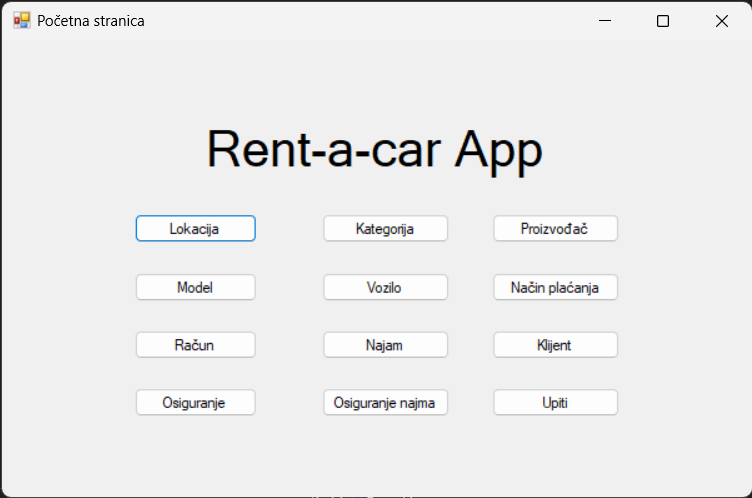
\includegraphics[width=0.9\textwidth]{slike/pocetna.png}
    \caption{Forma Početna stranica}
    \label{fig:pocetna}
\end{figure}

\subsection{Proizvođač}

\begin{figure}[!ht]
    \centering
    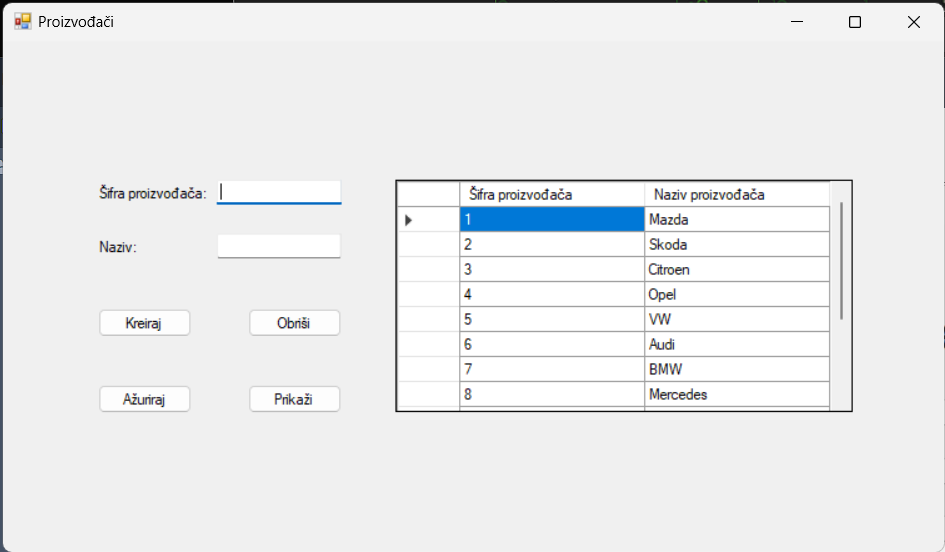
\includegraphics[width=0.9\textwidth]{slike/proizvodac.png}
    \caption{Forma Proizvođač}
    \label{fig:proizvodac}
\end{figure}
\newpage

\subsection{Račun}

\begin{figure}[!ht]
    \centering
    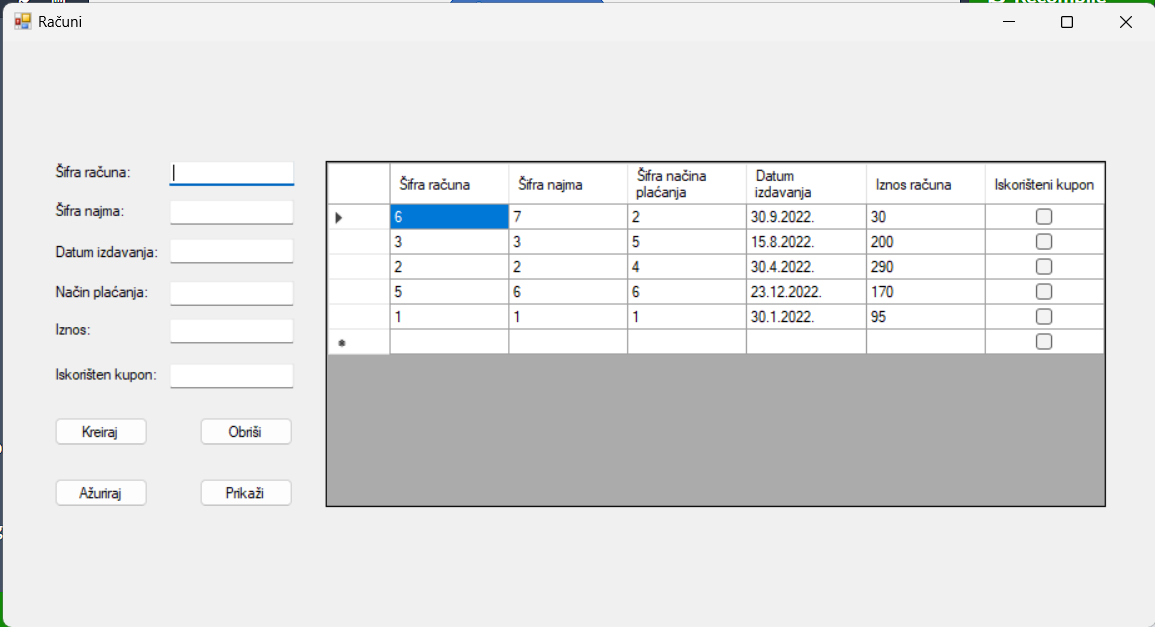
\includegraphics[width=0.9\textwidth]{slike/racun.png}
    \caption{Forma Račun}
    \label{fig:racun}
\end{figure}

\subsection{Vozilo}

\begin{figure}[!ht]
    \centering
    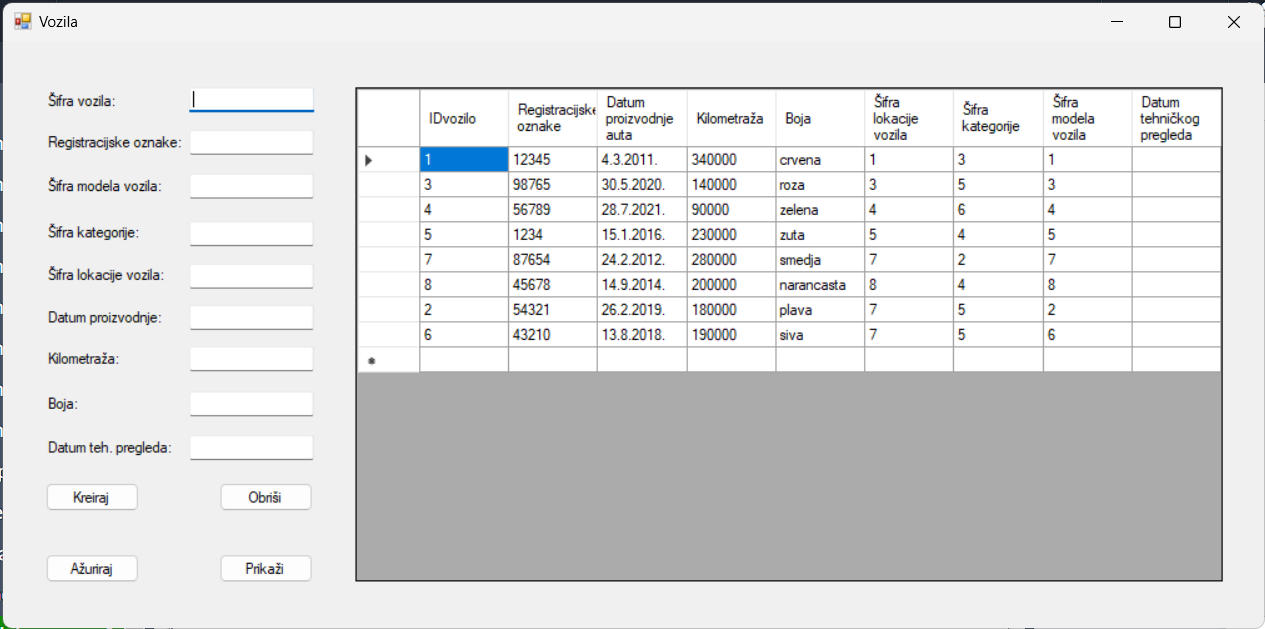
\includegraphics[width=0.9\textwidth]{slike/vozilo.png}
    \caption{Forma Vozilo}
    \label{fig:vozilo}
\end{figure}

\chapter{Zaključak}

Korišteni alati u ovom projektu su poprilično dobri za razvoj jednog ovakvog sustava. Prije svega, DataGrip je odličan alat koji omogućuje "profinjeno" kreiranje tablica, okidača, \textit{view}-ova. Izrada samog modela preko dijagrama je nešto teža, prije svega spajanje tablica vezama te kardinalnosti, ali sve u svemu, kada se smisli dobar konceptualni model sustava, tada izrada samog modela postaje linearan problem, točnije stvari se riješavaju jedna za drugom (slijedno).

Izrada same aplikacije u Visual Studiu također nije preteška. Sve \textit{Windows} forme se manje-više "crtaju", gumbići, \textit{label}-i, \textit{textbox}-ovi se \textit{drag and drop}-aju, zatim \textit{DataGridView}-ovi, koji su jako korisni, olakšavaju posao za tablični prikaz podataka, dok spajanje na bazu preko Npgsql providera također nije bio težak izazov.

Sama poslovna logika koja se temelji na razini baze preko aktivnih i temporalnih vrsta podataka, izrađena je preko funkcija i okidača. Izrada takvih vrsta baza podataka je bila nešto složenija i kompleksnija i tražila je poprilično jedan veći vremenski period u odnosu na prethodne "tehničke" izazove.

Navedene tehnologije za rad na ovakvom projektu su izabrane iz razloga zato što su zanimljive samom autoru ovog projekta, a i samim tim popularne u svijetu \textit{IT}-a te \textit{development}-a, točnije, naširoko su korištene, primjerice C\# koji je univerzalan i za sami \textit{frontend} i \textit{backend}, dok je PostgreSQL baza podataka korištena u \textit{large-scale} sustavima i tvrtkama.

\makebackmatter
% generira popis korištene literature, popis slika (ako je primjenjivo), popis tablica (ako je primjenjivo) i popis isječaka koda (ako je primjenjivo)

\appendices % ako nije potrebno, obrisati ili zakomentirati

\chapter{GitHub} % ako nije potrebno, obrisati ili zakomentirati

\href{https://github.com/pmatisic/rentacar}{Poveznica na repozitorij sustava za verzioniranje. (Potrebno je kliknuti na ovaj tekst.)}

\end{document}